\chapter{MÉTODOS E RECURSOS}
\label{cap:metodologia}
Este capítulo apresentará a visão geral dos passos para a execução do trabalho, assim como os métodos e ferramentas que serão utilizados.

\section{Visão Geral}

Para alcançar os objetivos propostos neste trabalho, será adotada uma abordagem metodológica que integrará pesquisa bibliográfica e pesquisa experimental, focando na comparação do desempenho de arquiteturas de detecção de objetos. A pesquisa terá caráter aplicado, com o objetivo de analisar métricas quantitativas de desempenho, como precisão, recall, mean Average Precision (mAP) e tempo de inferência, além de uma discussão crítica sobre a aplicabilidade de cada modelo em diferentes cenários.

O processo metodológico poderá ser visualizado no fluxograma da \autoref{fig:fluxograma}. Ele se iniciará com o estudo teórico e a revisão bibliográfica, seguido pela seleção de modelos, que incluirão YOLO, Faster R-CNN, SSD, EfficientDet e RetinaNet. Em seguida, serão selecionados e pré-processados os datasets, como o COCO Dataset, PASCAL VOC Dataset e Kaggle Dataset. A pesquisa prosseguirá com a configuração do ambiente (TensorFlow) e a definição do hardware. Após a definição e otimização dos hiperparâmetros, os modelos serão treinados. A inferência será realizada com um conjunto de teste, as métricas de desempenho serão coletadas, e os resultados serão comparados e analisados quantitativamente. O processo se encerrará com a análise crítica e a discussão dos modelos, seguida da conclusão e sugestões para trabalhos futuros.

\begin{figure}[H]
\caption{Diagrama de processos do desenvolvimento do TCC}
\centering
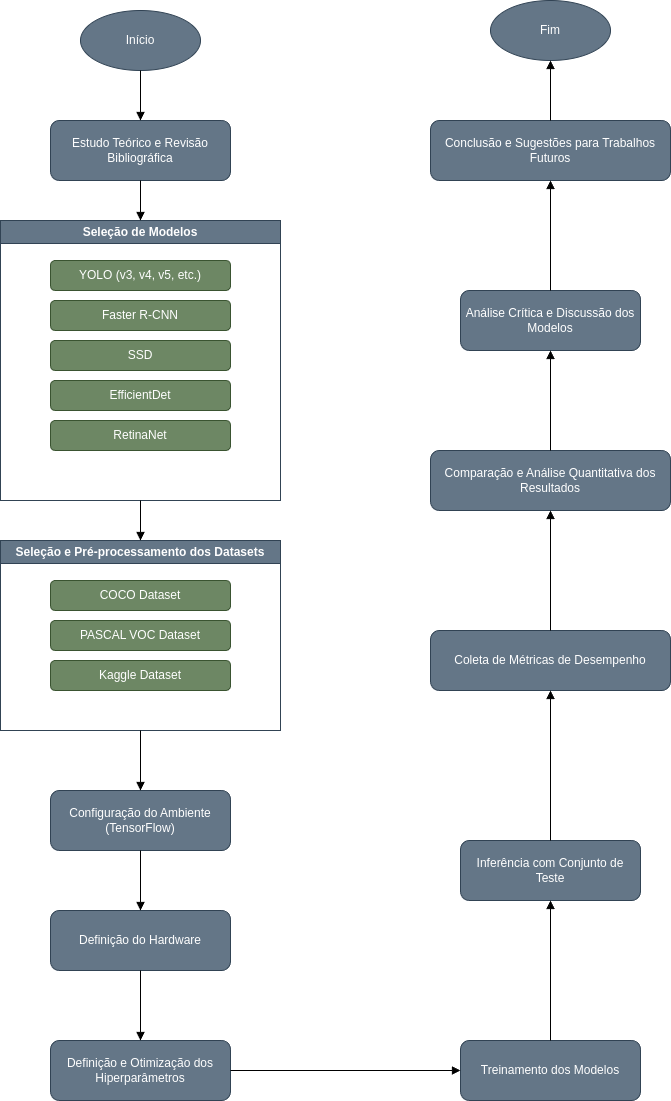
\includegraphics[width=0.8\textwidth]{media/fluxograma.png}
\fonte{Elaborado pelo autor (2025)}
\label{fig:fluxograma}
\end{figure}

\section{Estudo Teórico e Revisão Bibliográfica}

Nesta etapa, será realizado um estudo aprofundado sobre os fundamentos da visão computacional e do aprendizado de máquina, com foco em redes neurais de aprendizagem profunda. Serão revisados os conceitos e as arquiteturas de detecção de objetos mais relevantes, como YOLO, Faster R-CNN, SSD, EfficientDet e RetinaNet. Esta fase buscará fundamentar teoricamente a pesquisa, compreendendo as características, vantagens e limitações de cada modelo.

\section{Seleção e Pré-processamento dos Datasets}

Serão selecionados e pré-processados os principais datasets de referência para detecção de objetos, como o COCO Dataset, PASCAL VOC Dataset e Kaggle Dataset. O pré-processamento envolverá a preparação e organização dos dados para o treinamento dos modelos.

\section{Configuração do Ambiente e Definição do Hardware}

A configuração do ambiente de desenvolvimento será feita utilizando o framework TensorFlow. O Google Colab, com runtime que utiliza placa de vídeo dedicada, será empregado para o treinamento dos modelos, devido à sua acessibilidade e capacidade de processamento. Serão definidos os requisitos de hardware, levando em consideração as necessidades computacionais de cada modelo para o treinamento e inferência.

\section{Definição e Otimização dos Hiperparâmetros}

Nesta etapa, serão definidos e otimizados os hiperparâmetros de cada modelo para garantir o melhor desempenho possível durante o treinamento. Este processo é crucial para ajustar os modelos aos datasets e ao hardware disponível.

\section{Treinamento e Inferência dos Modelos}

Os modelos de detecção de objetos serão treinados com os datasets pré-processados. Após o treinamento, a inferência será realizada em um conjunto de testes para avaliar o desempenho de cada modelo em dados não vistos.

\section{Coleta de Métricas e Análise de Resultados}

Serão coletadas métricas de desempenho, como precisão, recall, mean Average Precision (mAP) e tempo de inferência. Os resultados serão comparados e analisados quantitativamente para identificar o equilíbrio entre precisão e velocidade de cada arquitetura.

\section{Análise Crítica e Discussão dos Modelos}

Com base na análise quantitativa, será realizada uma discussão crítica sobre o desempenho de cada modelo. Esta etapa considerará não apenas as métricas, mas também a complexidade de implementação e a escalabilidade, fornecendo subsídios para a escolha do algoritmo mais adequado a cada contexto.

\section{Conclusão e Sugestões para Trabalhos Futuros}

Por fim, o trabalho apresentará uma conclusão sobre os resultados obtidos e as principais contribuições da pesquisa. Serão feitas sugestões para trabalhos futuros, explorando possíveis melhorias e novas direções para a área de detecção de objetos.